\documentclass[]{article}
\usepackage{lmodern}
\usepackage{amssymb,amsmath}
\usepackage{ifxetex,ifluatex}
\usepackage{fixltx2e} % provides \textsubscript
\ifnum 0\ifxetex 1\fi\ifluatex 1\fi=0 % if pdftex
  \usepackage[T1]{fontenc}
  \usepackage[utf8]{inputenc}
\else % if luatex or xelatex
  \ifxetex
    \usepackage{mathspec}
  \else
    \usepackage{fontspec}
  \fi
  \defaultfontfeatures{Ligatures=TeX,Scale=MatchLowercase}
\fi
% use upquote if available, for straight quotes in verbatim environments
\IfFileExists{upquote.sty}{\usepackage{upquote}}{}
% use microtype if available
\IfFileExists{microtype.sty}{%
\usepackage{microtype}
\UseMicrotypeSet[protrusion]{basicmath} % disable protrusion for tt fonts
}{}
\usepackage[margin=1in]{geometry}
\usepackage{hyperref}
\hypersetup{unicode=true,
            pdftitle={ID5059 - P1 - Auto MPG Analysis},
            pdfauthor={180024570},
            pdfborder={0 0 0},
            breaklinks=true}
\urlstyle{same}  % don't use monospace font for urls
\usepackage{graphicx,grffile}
\makeatletter
\def\maxwidth{\ifdim\Gin@nat@width>\linewidth\linewidth\else\Gin@nat@width\fi}
\def\maxheight{\ifdim\Gin@nat@height>\textheight\textheight\else\Gin@nat@height\fi}
\makeatother
% Scale images if necessary, so that they will not overflow the page
% margins by default, and it is still possible to overwrite the defaults
% using explicit options in \includegraphics[width, height, ...]{}
\setkeys{Gin}{width=\maxwidth,height=\maxheight,keepaspectratio}
\IfFileExists{parskip.sty}{%
\usepackage{parskip}
}{% else
\setlength{\parindent}{0pt}
\setlength{\parskip}{6pt plus 2pt minus 1pt}
}
\setlength{\emergencystretch}{3em}  % prevent overfull lines
\providecommand{\tightlist}{%
  \setlength{\itemsep}{0pt}\setlength{\parskip}{0pt}}
\setcounter{secnumdepth}{5}
% Redefines (sub)paragraphs to behave more like sections
\ifx\paragraph\undefined\else
\let\oldparagraph\paragraph
\renewcommand{\paragraph}[1]{\oldparagraph{#1}\mbox{}}
\fi
\ifx\subparagraph\undefined\else
\let\oldsubparagraph\subparagraph
\renewcommand{\subparagraph}[1]{\oldsubparagraph{#1}\mbox{}}
\fi

%%% Use protect on footnotes to avoid problems with footnotes in titles
\let\rmarkdownfootnote\footnote%
\def\footnote{\protect\rmarkdownfootnote}

%%% Change title format to be more compact
\usepackage{titling}

% Create subtitle command for use in maketitle
\newcommand{\subtitle}[1]{
  \posttitle{
    \begin{center}\large#1\end{center}
    }
}

\setlength{\droptitle}{-2em}

  \title{ID5059 - P1 - Auto MPG Analysis}
    \pretitle{\vspace{\droptitle}\centering\huge}
  \posttitle{\par}
  \subtitle{MSc Data-Intensive Analysis}
  \author{180024570}
    \preauthor{\centering\large\emph}
  \postauthor{\par}
      \predate{\centering\large\emph}
  \postdate{\par}
    \date{04/03/2019}

\usepackage{subfig}
\usepackage{booktabs}
\usepackage{longtable}
\usepackage{array}
\usepackage{multirow}
\usepackage[table]{xcolor}
\usepackage{wrapfig}
\usepackage{float}
\usepackage{colortbl}
\usepackage{pdflscape}
\usepackage{tabu}
\usepackage{threeparttable}
\usepackage{threeparttablex}
\usepackage[normalem]{ulem}
\usepackage{makecell}

\usepackage{booktabs} \usepackage{longtable} \usepackage{array} \usepackage{enumitem} \usepackage{multirow} \usepackage[table]{xcolor} \usepackage{wrapfig} \usepackage{float} \floatplacement{figure}{H} \usepackage[bottom]{footmisc}

\begin{document}
\maketitle

{
\setcounter{tocdepth}{2}
\tableofcontents
}
\emph{I confirm that the following report and associated code is my own
work, except where clearly indicated.}

\hypertarget{introduction}{%
\section{Introduction}\label{introduction}}

This practical analyse the pairwise relationships of MPG against
Displacement, Horsepower, Weight and Acceleration. Linear models
(section 2), bin smooth models (section 3) and B-spline models (section
5) are implemented based on each of the four predictors. The fit of
these models is evaluated by RSS, AIC and a measure of generalisation
error, Mean Squred Error of prediction of test data.

\begin{quote}
Orange line is the minimum. 6 observations without hoursepower values
are omitted in this analysis.
\end{quote}

\hypertarget{linear-models}{%
\section{Linear Models}\label{linear-models}}

In this section, linear models are implemented using Displacement,
Horsepower, Weight and Acceleration to predict MPG. The candidates
models for each predictor are based on polynomial terms with degree from
1 to 15. RSS, AIC and MSE of 10-fold cross validation are used as
measurement of model fitting.

\hypertarget{linear-models-for-displacement}{%
\subsection{Linear Models for
Displacement}\label{linear-models-for-displacement}}

\begin{figure}

{\centering 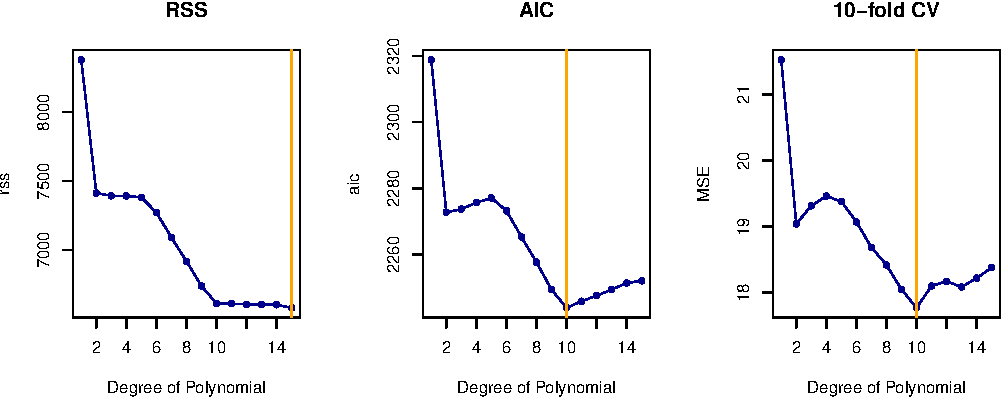
\includegraphics{Report_files/figure-latex/lm-disp-1} 

}

\caption{Candidate Linear Models for Displacement}\label{fig:lm-disp}
\end{figure}

Figure 1 shows the evaluation of 15 candidate models in terms of three
measurement. \emph{RSS}, \emph{AIC} and \emph{MSE} of 10-fold cross
validation appear to have similar trends when the degree lower than 10.
\emph{RSS} continues to gently decline after that, but \emph{AIC} and
\emph{MSE} start rising because of overfitting.

Therefore, the one with degree 10 is selected and shown in figure 2.

\begin{figure}

{\centering 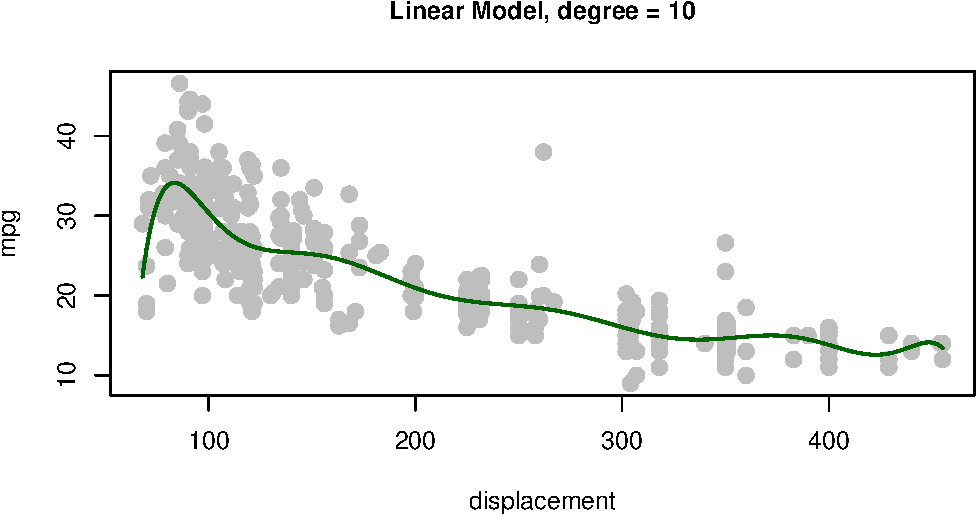
\includegraphics{Report_files/figure-latex/lm-d-best-1} 

}

\caption{Selected Linear Models for Displacement}\label{fig:lm-d-best}
\end{figure}

RSS: 6610.19 AIC: 2243.889 MSE: 17.68683

\hypertarget{linear-models-for-horsepower}{%
\subsection{Linear Models for
Horsepower}\label{linear-models-for-horsepower}}

\begin{figure}

{\centering 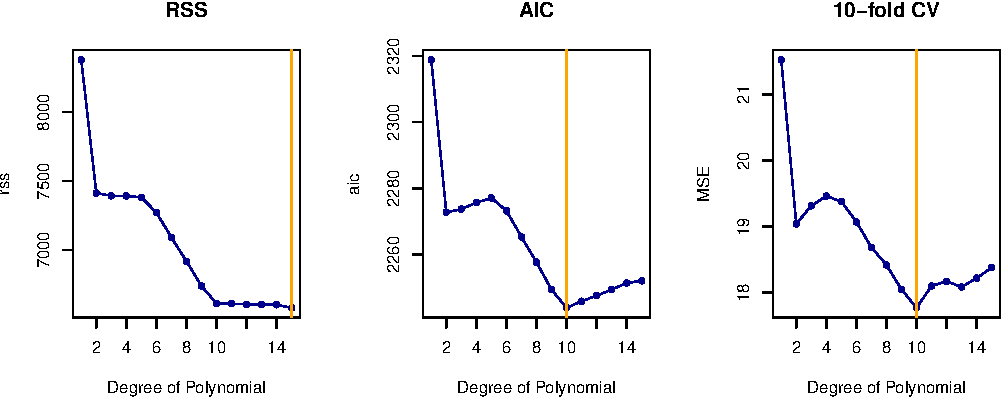
\includegraphics{Report_files/figure-latex/lm-h-1} 

}

\caption{Candidate Linear Models for Horsepower}\label{fig:lm-h}
\end{figure}

Similar to Displacement, figure 3 shows the optimal model for Horsepower
is also with degree 10. The model is illustrated in figure 4.

\begin{figure}

{\centering 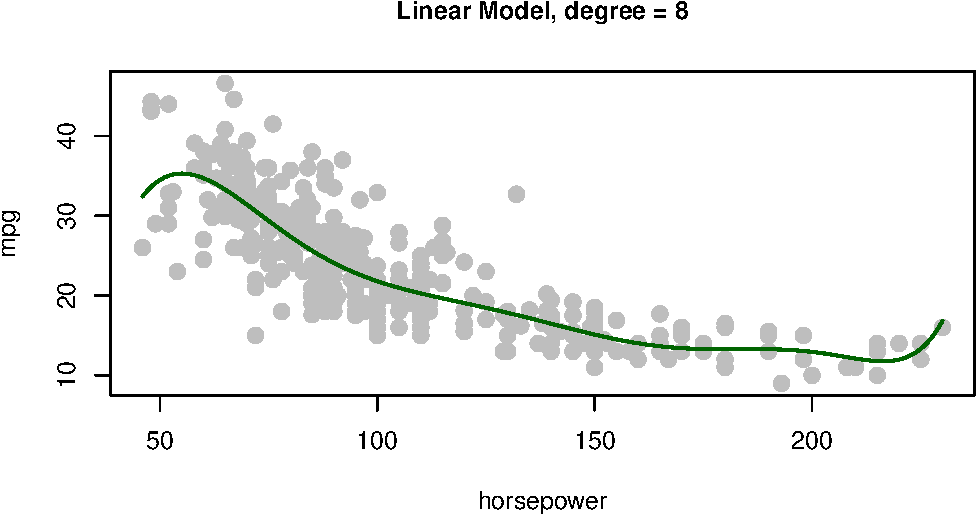
\includegraphics{Report_files/figure-latex/lm-h-best-1} 

}

\caption{Selected Linear Models for Horsepower}\label{fig:lm-h-best}
\end{figure}

RSS: 7081.923 AIC: 2266.911 MSE: 18.83704

\hypertarget{linear-models-for-weight}{%
\subsection{Linear Models for Weight}\label{linear-models-for-weight}}

\begin{figure}

{\centering 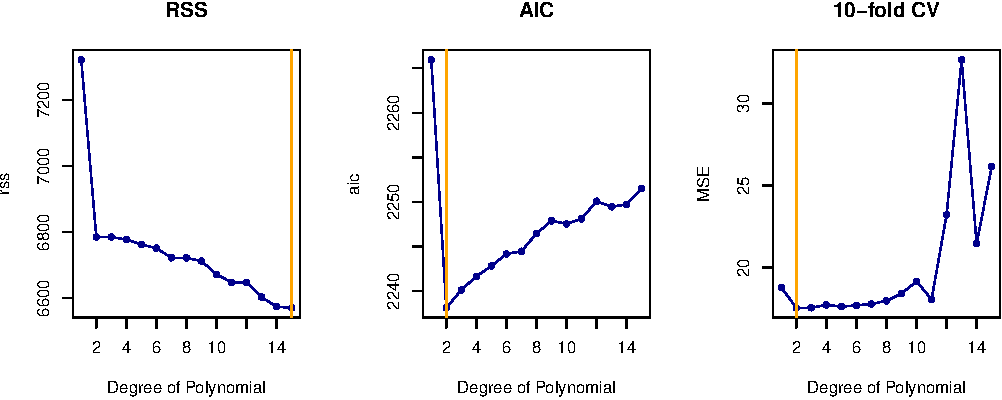
\includegraphics{Report_files/figure-latex/lm-w-1} 

}

\caption{Candidate Linear Models for Weight}\label{fig:lm-w}
\end{figure}

Figure 5 illustrates that the linear models created using Weight have
different trends from the previous two. The generalisation errors based
on 10-fold cross validation show slight variation between degree 2 and
8, while AIC score shows a steep fall from degree 1 to 2 and then
steadily increace.

The optimal model for Weight, shown in figure 6, is selected to be the
one with polynomial degree equal to 2.

\begin{figure}

{\centering 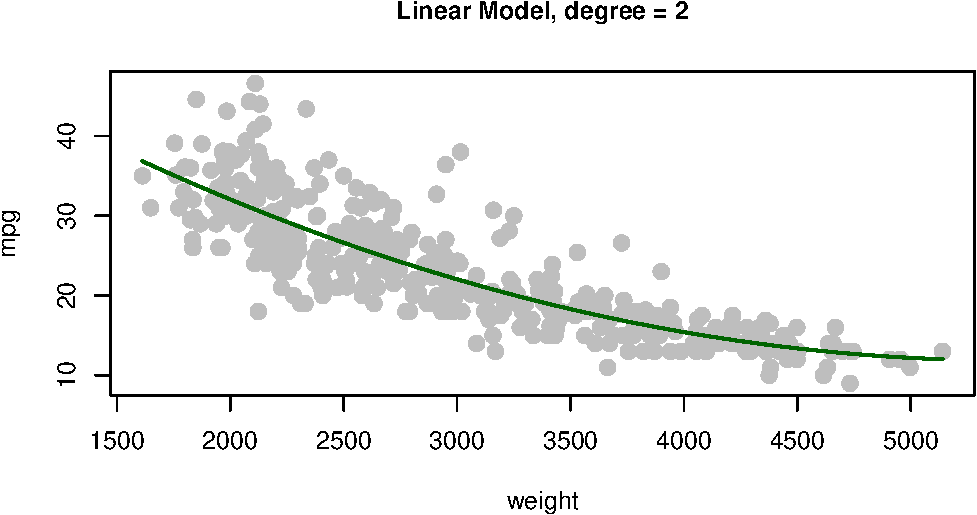
\includegraphics{Report_files/figure-latex/lm-w-best-1} 

}

\caption{Selected Linear Models for Weight}\label{fig:lm-w-best}
\end{figure}

RSS: 6784.899 AIC: 2238.115 MSE: 17.43871

\hypertarget{linear-models-for-acceleration}{%
\subsection{Linear Models for
Acceleration}\label{linear-models-for-acceleration}}

\begin{figure}

{\centering 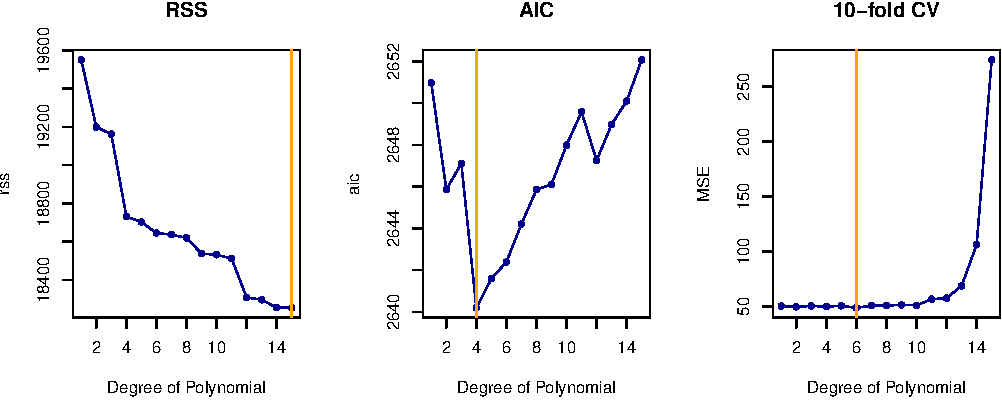
\includegraphics{Report_files/figure-latex/lm-a-1} 

}

\caption{Candidate Linear Models for Acceleration}\label{fig:lm-a}
\end{figure}

According to figure 7, the MSE barely varies from degree 1 to 10, but
the error values are considerably larger than all the previous. The
optimal model for Acceleration is selected to be the one with the lowest
AIC score, degree equal to 4 and shown in figure 8.

\begin{figure}

{\centering 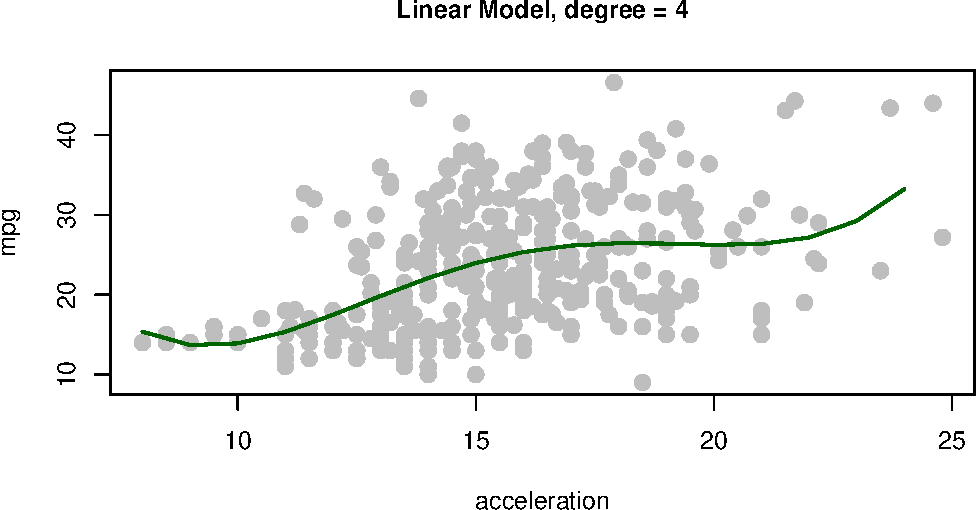
\includegraphics{Report_files/figure-latex/lm-a-best-1} 

}

\caption{Selected Linear Models for Acceleration}\label{fig:lm-a-best}
\end{figure}

RSS: 18731.31 AIC: 2640.19 MSE: 49.24686

\hypertarget{summary-for-linear-models}{%
\subsection{Summary for Linear Models}\label{summary-for-linear-models}}

On the basis of the linear models implemented in the section, it is easy
to conclude that the \emph{Residual Sum of Square} monotonically
decreases with the increase of model comlexity, namely the degree of
polynomial terms in this case. As to \emph{Akaike information
criterion}, the penalty on the number of model parameters would
outweight the benefits of model complexity beyond a certain degree.
\emph{Mean Squard Error} based on cross validation will also increase
when the model is overfitting.

\begin{longtable}[t]{lrrr}
\caption{\label{tab:lm-sum}Summary of Model Fitting Measurement for the Selected Linear Model}\\
\toprule
  & RSS & AIC & MSE\\
\midrule
Displacement & 6610.19 & 2243.89 & 17.69\\
Horsepower & 7081.92 & 2266.91 & 18.84\\
Weight & 6784.90 & 2238.12 & 17.44\\
Acceleration & 18731.31 & 2640.19 & 49.25\\
\bottomrule
\end{longtable}

Table 1 summarises the evaluation for the four optimal model based on
Displacement, Horsepower, Weight and Acceleration. It's clear that the
Acceleration model is the is far worse than the other three. Overall,
the Displacement model and the Weight are as good at predition, while
the Weight model with 2 degree is much simpler than degree 10 of the
Displacement model.

\hypertarget{bin-smooth-models}{%
\section{Bin Smooth Models}\label{bin-smooth-models}}

Dataset is randomly split into two halves (each has 196 observations) in
this section, one used as training data to fit models and the other as
test data to obtain generalisation error. Four predictors are fitted
into bin smoorh models, and candidate models for each predictor are
across bin length from 1 to 200. One optimal bin smooth model with the
most reasonable bin length is selected for each predictor, and the four
selected models competes with each other.

\hypertarget{bin-smooth-models-for-displacement}{%
\subsection{Bin Smooth Models for
Displacement}\label{bin-smooth-models-for-displacement}}

\begin{figure}

{\centering 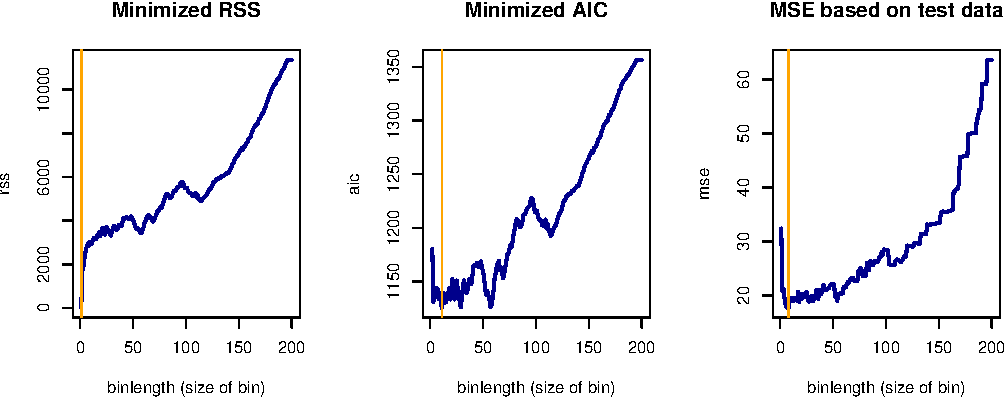
\includegraphics{Report_files/figure-latex/bin-d-1} 

}

\caption{Candidate Bin Smooth Models for Displacement}\label{fig:bin-d}
\end{figure}

Bin lenght: 10 Number of bins: 20 RSS: 2963.098 AIC: 1130.536 MSE:
19.44981

\begin{figure}

{\centering 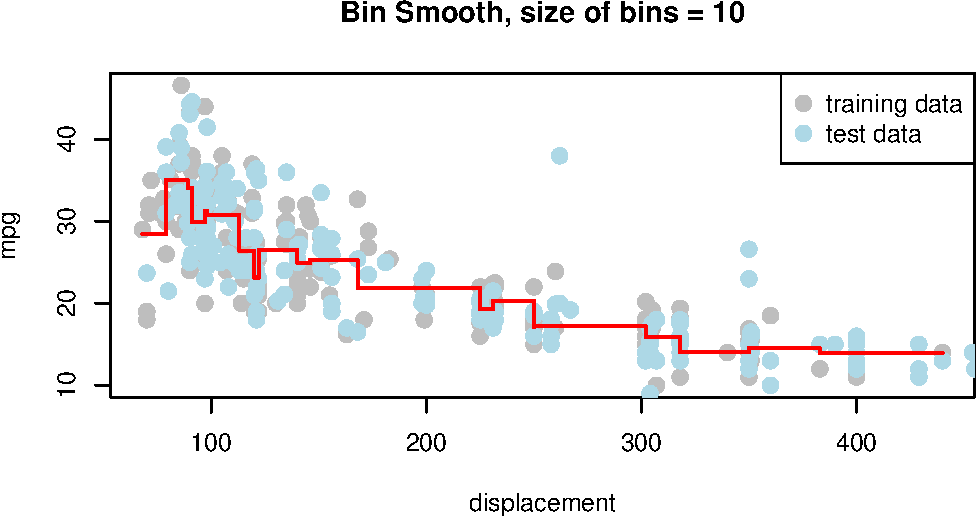
\includegraphics{Report_files/figure-latex/bin-d-best-1} 

}

\caption{Selected Bin Smooth Models for Displacement}\label{fig:bin-d-best}
\end{figure}

Figure 9 shows the most reasonable bin length is around 10, and figure
10 illustrates the optimal bin smooth model for predictor Displacement.

\hypertarget{bin-smooth-models-for-horsepower}{%
\subsection{Bin Smooth Models for
Horsepower}\label{bin-smooth-models-for-horsepower}}

\begin{figure}

{\centering 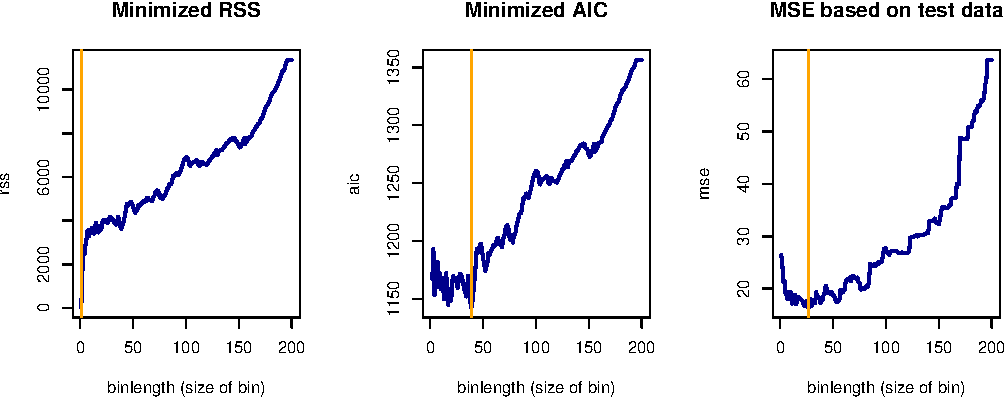
\includegraphics{Report_files/figure-latex/bin-h-1} 

}

\caption{Candidate Bin Smooth Models for Horsepower}\label{fig:bin-h}
\end{figure}

Bin lenght: 20 Number of bins: 10 RSS: 3415.697 AIC: 1138.396 MSE:
20.30473

\begin{figure}

{\centering 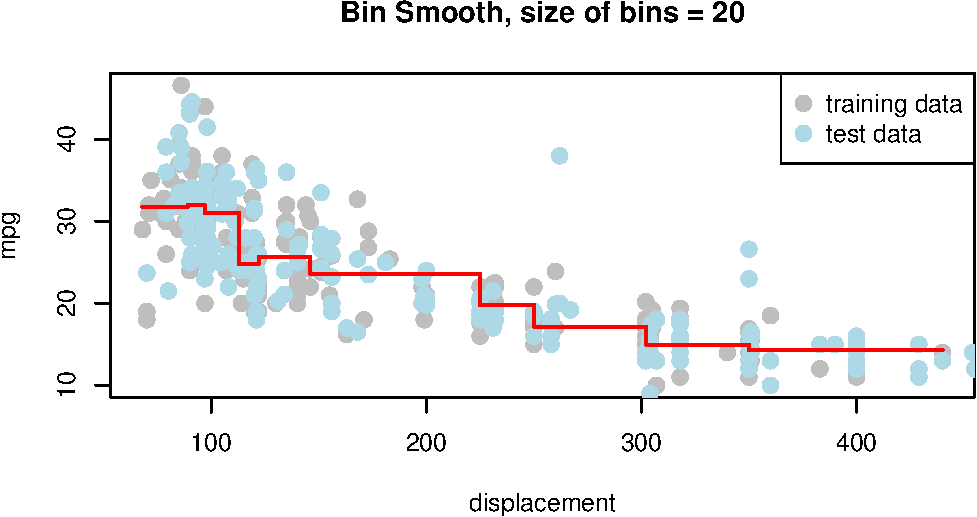
\includegraphics{Report_files/figure-latex/bin-h-best-1} 

}

\caption{Selected Bin Smooth Models for Horsepower}\label{fig:bin-h-best}
\end{figure}

Figure 11 shows the most reasonable bin length fall between 10 - 40, and
figure 12 illustrates the selected optimal bin smooth model for
predictor Horsepower, with bin length equal to 20.

\hypertarget{bin-smooth-models-for-weight}{%
\subsection{Bin Smooth Models for
Weight}\label{bin-smooth-models-for-weight}}

\begin{figure}

{\centering 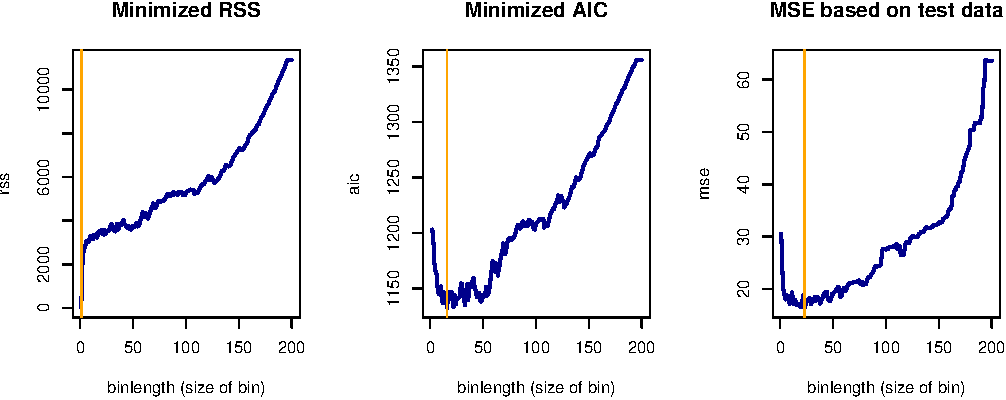
\includegraphics{Report_files/figure-latex/bin-w-1} 

}

\caption{Candidate Bin Smooth Models for Weight}\label{fig:bin-w}
\end{figure}

Bin lenght: 20 Number of bins: 10 RSS: 3563.595 AIC: 1146.704 MSE:
17.32378

\begin{figure}

{\centering 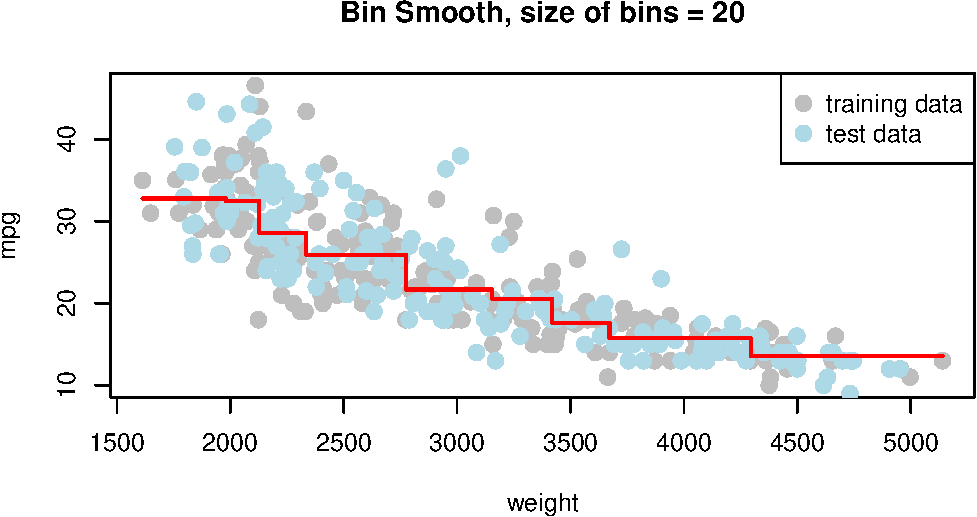
\includegraphics{Report_files/figure-latex/bin-w-best-1} 

}

\caption{Selected Bin Smooth Models for Weight}\label{fig:bin-w-best}
\end{figure}

Figure 13 shows the most reasonable bin length fall between 10 - 30, and
figure 14 illustrates the selected optimal bin smooth model for
predictor Weight, with bin length equal to 20.

\hypertarget{bin-smooth-models-for-acceleration}{%
\subsection{Bin Smooth Models for
Acceleration}\label{bin-smooth-models-for-acceleration}}

\begin{figure}

{\centering 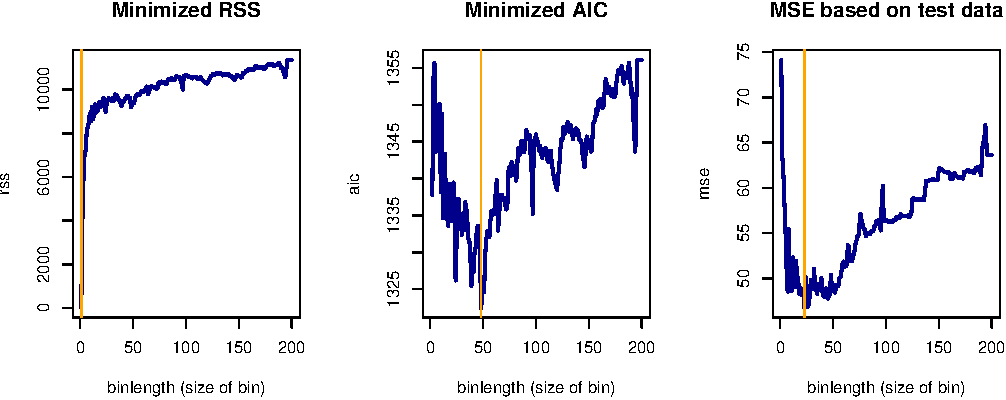
\includegraphics{Report_files/figure-latex/bin-a-1} 

}

\caption{Candidate Bin Smooth Models for Acceleration}\label{fig:bin-a}
\end{figure}

Bin lenght: 25 Number of bins: 8 RSS: 9339.012 AIC: 1331.537 MSE:
48.09347

\begin{figure}

{\centering 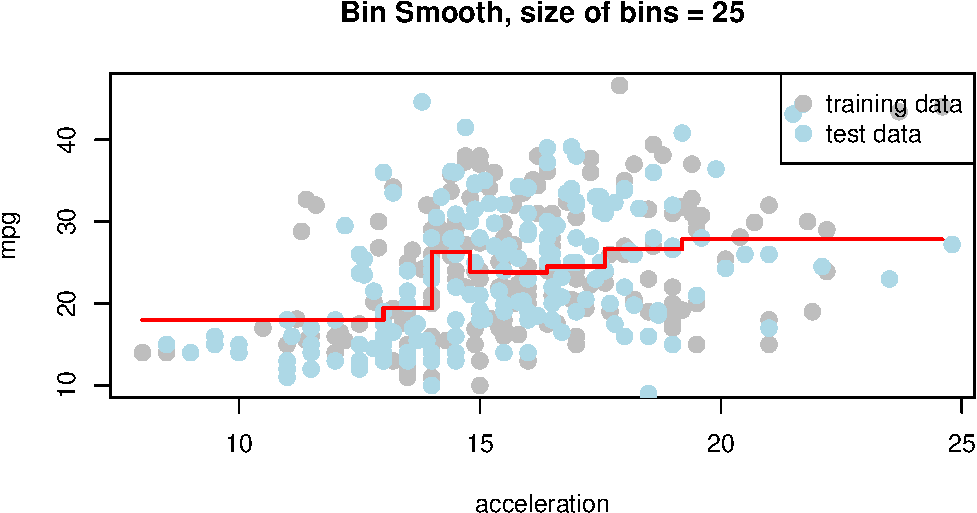
\includegraphics{Report_files/figure-latex/bin-a-best-1} 

}

\caption{Selected Bin Smooth Models for Acceleration}\label{fig:bin-a-best}
\end{figure}

Figure 15 shows that the \emph{AIC} and \emph{MSE} lines are way more
wiggly than all the previous, which indicates the smooth models for
Acceleration have much uncertainty than others. And similar to linear
model section, the \emph{AIC} and \emph{RSS} are also reletively higher
than models based on other three predictors.

Figure 16 illustrates the selected optimal bin smooth model for
predictor Acceleration, with bin length equal to 25.

\hypertarget{summary-for-bin-smooth-models}{%
\subsection{Summary for Bin Smooth
Models}\label{summary-for-bin-smooth-models}}

The most obvious pattern within bin smooth models is that decreasing the
number of bins (increasing the size) would increase \emph{RSS}, and
increasing the number of bins (reducing the size) would lessen
\emph{RSS}. Generally, four groups of models all show better predictive
ability at smaller bin length than at large bin length. However, excess
of bins (namely bin length too small) usually leads to overfitting,
despite the lower \emph{RSS}.

\begin{longtable}[t]{lrrrr}
\caption{\label{tab:bin-sum}Summary of Model Fitting Measurement for the Selected Bin Smooth Model}\\
\toprule
  & RSS & AIC & MSE & Adjusted R2\\
\midrule
Displacement & 2963.10 & 1130.54 & 19.45 & 0.71\\
Horsepower & 3415.70 & 1138.40 & 20.30 & 0.69\\
Weight & 3563.60 & 1146.70 & 17.32 & 0.67\\
Acceleration & 9339.01 & 1331.54 & 48.09 & 0.15\\
\bottomrule
\end{longtable}

The measurements of four optimal models are summarized below in table 2.
\emph{AIC} scores of bin smooth models are around 1000, clearly lower
than those of linear models (around 2000), because bin smooth model is
simpler than high degree linear regression model. Acceleration is still
the worst predictor, the three other models have similar predictive
abilities. Displacement model outdo other three models in terms of
\emph{RSS}, \emph{AIC} and adjusted \(R^2\), but the generalisation
error (\emph{MSE}) is slightly higher than of Weight model.

\hypertarget{b-spline-models}{%
\section{B-spline Models}\label{b-spline-models}}

In this section, four predictors are respectively fitted to four group
of b-spline models. There are 30 candidate models in each group, with
the number of knots from 1 to 10 and degree from 1 to 3. The knots are
placed in a uniform fashion. One optimal model is selected for each
group/predictor, and four optimal b-spline model compete. The training
data and test data are the same as used in the last section. The
generalisation error is the \emph{MSE} of prediction on test data.

\hypertarget{b-spline-models-for-displacement}{%
\subsection{B-spline Models for
Displacement}\label{b-spline-models-for-displacement}}

\begin{figure}

{\centering 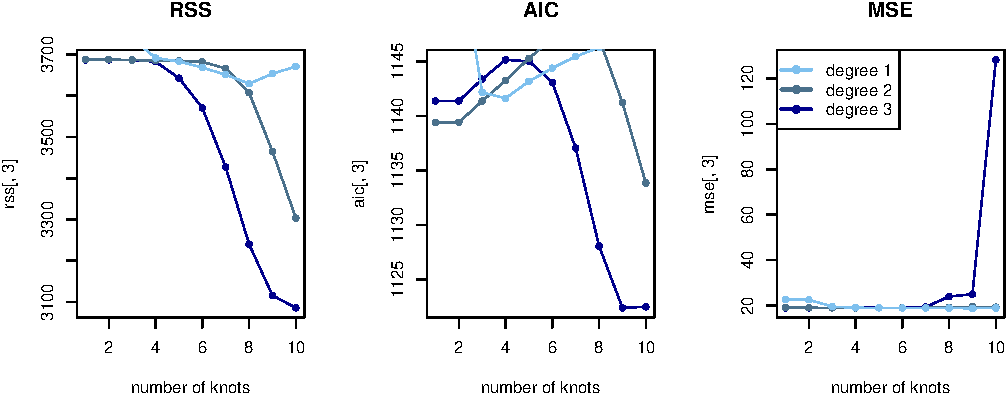
\includegraphics{Report_files/figure-latex/bs-d-1} 

}

\caption{Candidate B-spline Models for Displacement}\label{fig:bs-d}
\end{figure}

Figure 17 shows that degree 3 models have loewr \emph{RSS} than models
with degree 1 and 2, and \emph{AIC} scores are also lower when the
number of knots exceeding 6. However, degree 3 models highly diverge
with large number of knots, resulting extreme generalisation errors.

The optimal b-spline model for Displacement is selected to be the one
with 7 knots and degree equal to 3, shown in figure 18. The vertical
dotted lines indicate positions of the knots. (hereafter the same)

\begin{figure}

{\centering 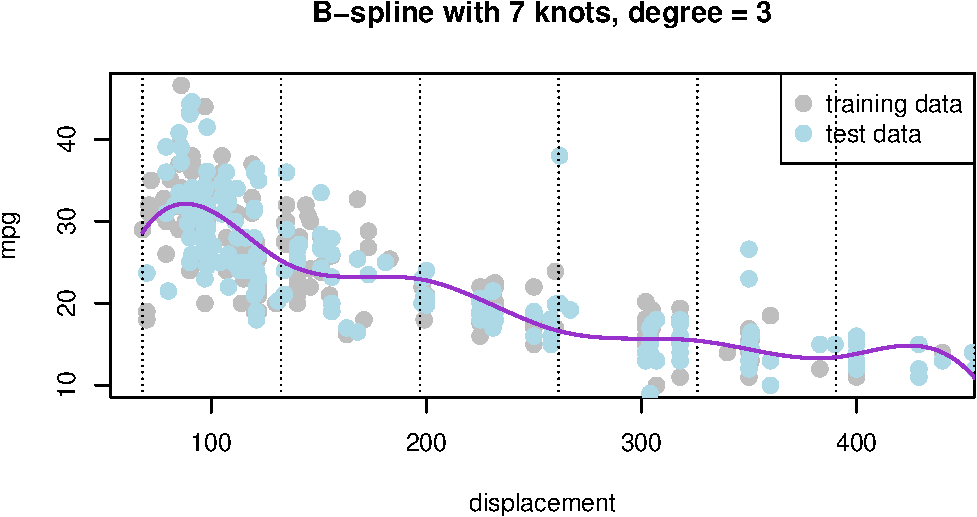
\includegraphics{Report_files/figure-latex/bs-d-opt-1} 

}

\caption{Selected B-spline Models for Displacement}\label{fig:bs-d-opt}
\end{figure}

RSS: 3426.912 AIC: 1137.039 MSE: 19.3498

\hypertarget{b-spline-models-for-horsepower}{%
\subsection{B-spline Models for
Horsepower}\label{b-spline-models-for-horsepower}}

\begin{figure}

{\centering 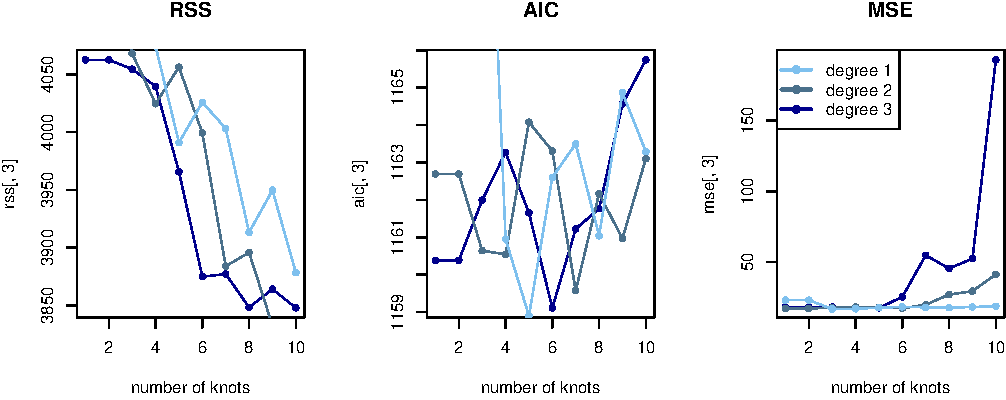
\includegraphics{Report_files/figure-latex/bs-h-1} 

}

\caption{Candidate B-spline Models for Horsepower}\label{fig:bs-h}
\end{figure}

Figure 19 shows that \emph{RSS} of degree 3 models are generally lower
than others but \emph{MSE} diverge since the number of knots surpass 5.
The \emph{AIC} plot seems jumbled up, but the fluctuation range is
generally within 5, not problematic.

The optimal b-spline model for Horsepower is selected to be the one with
5 knots and degree equal to 3, shown in figure 20.

\begin{figure}

{\centering 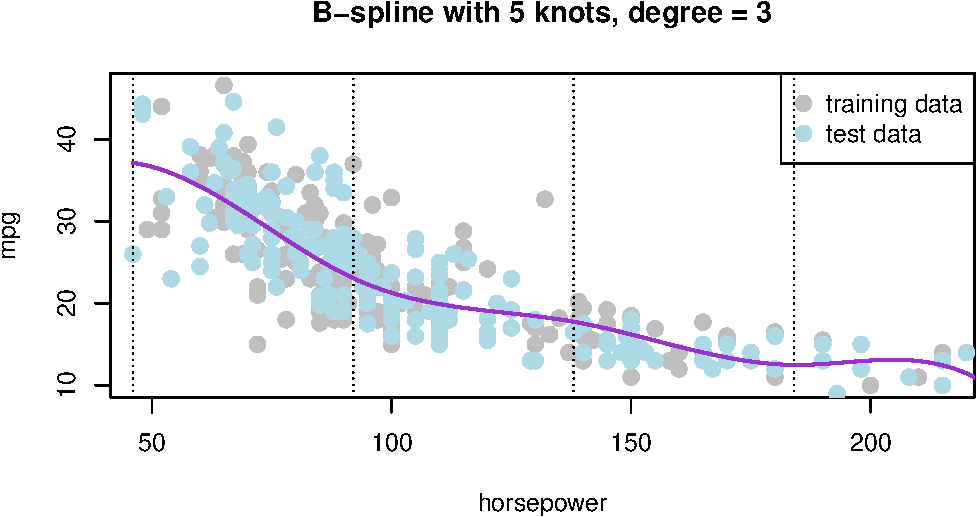
\includegraphics{Report_files/figure-latex/bs-h-opt-1} 

}

\caption{Selected B-spline Models for Horsepower}\label{fig:bs-h-opt}
\end{figure}

RSS: 3965.61 AIC: 1161.655 MSE: 17.69047

\hypertarget{b-spline-models-for-weight}{%
\subsection{B-spline Models for
Weight}\label{b-spline-models-for-weight}}

\begin{figure}

{\centering 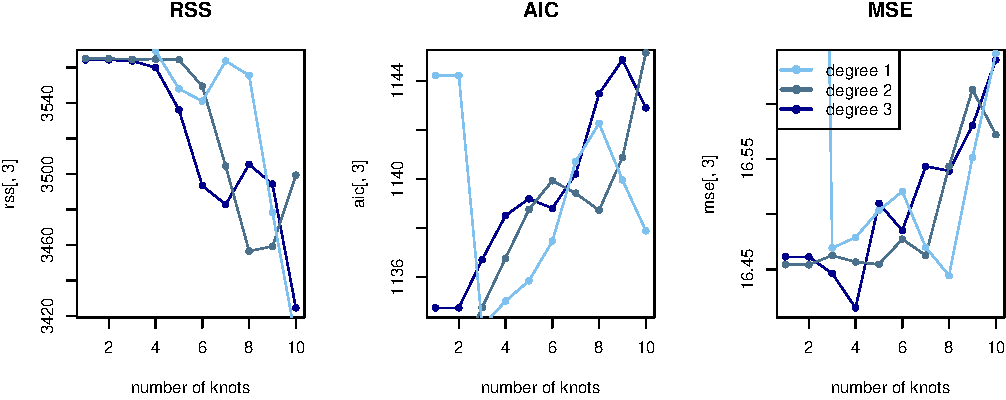
\includegraphics{Report_files/figure-latex/bs-w-1} 

}

\caption{Candidate B-spline Models for Weight}\label{fig:bs-w}
\end{figure}

Figure 21 shows that \emph{AIC} and \emph{MSE} trend to increase after
number of knots surpass 3 and 4. The optimal b-spline model for Weight
is selected to be the one with 4 knots and degree equal to 3, shown in
figure 22.

\begin{figure}

{\centering 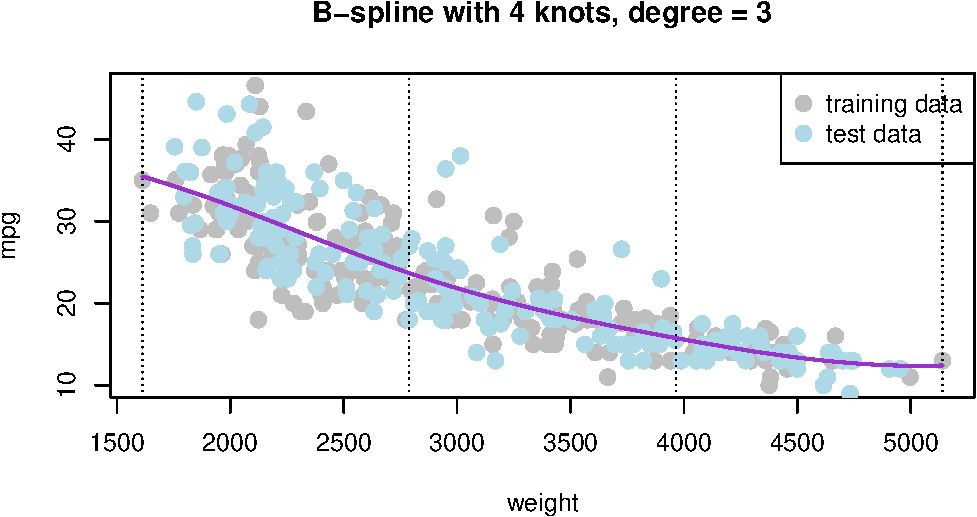
\includegraphics{Report_files/figure-latex/bs-w-opt-1} 

}

\caption{Selected B-spline Models for Weight}\label{fig:bs-w-opt}
\end{figure}

RSS: 3560.09 AIC: 1138.512 MSE: 16.41512

\hypertarget{b-spline-models-for-acceleration}{%
\subsection{B-spline Models for
Acceleration}\label{b-spline-models-for-acceleration}}

\begin{figure}

{\centering 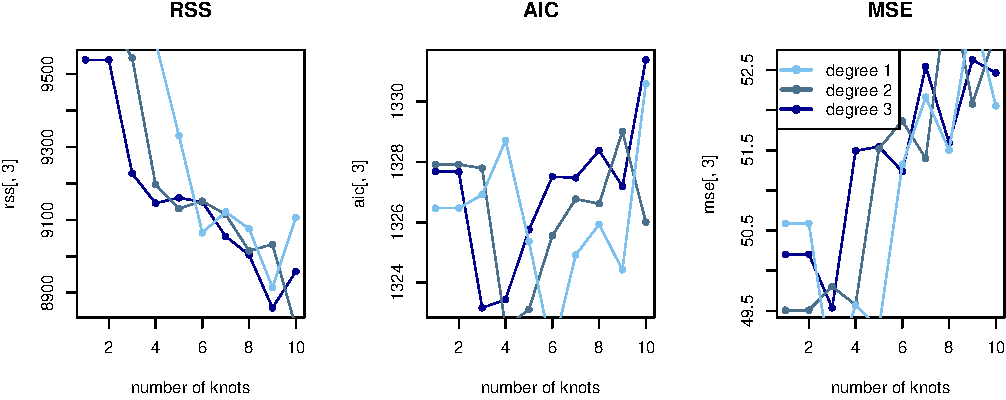
\includegraphics{Report_files/figure-latex/bs-a-1} 

}

\caption{Candidate B-spline Models for Acceleration}\label{fig:bs-a}
\end{figure}

Figure 23 shows that there is not much difference between models with
three degrees. The optimal b-spline model for Weight is selected to be
the one with 4 knots and degree equal to 2, shown in figure 24.

\begin{figure}

{\centering 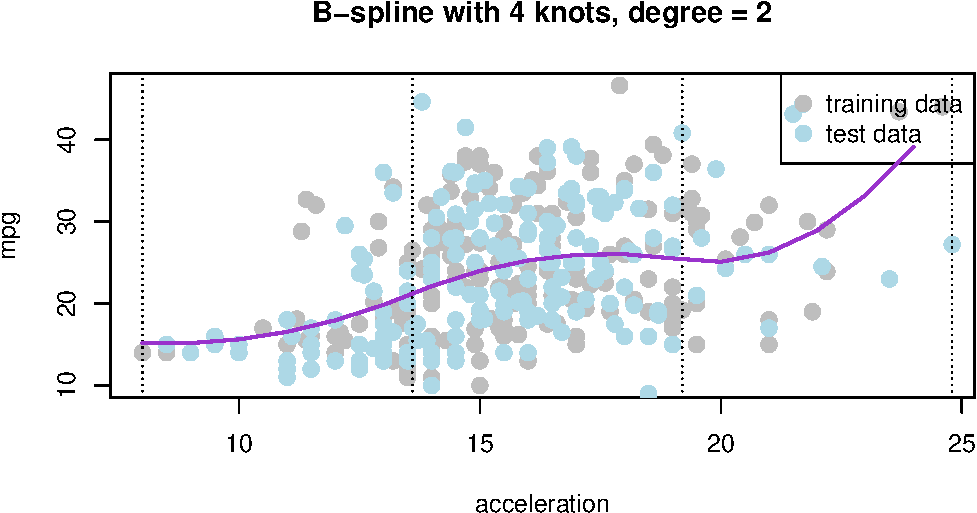
\includegraphics{Report_files/figure-latex/bs-a-opt-1} 

}

\caption{Selected B-spline Models for Acceleration}\label{fig:bs-a-opt}
\end{figure}

RSS: 9196.567 AIC: 1322.524 MSE: 49.57517

\hypertarget{summary-for-b-spline-models}{%
\subsection{Summary for B-spline
Models}\label{summary-for-b-spline-models}}

Generally, the number of knots and degree of polynomial determine the
flexibility of the model: the more the knots, the more flexible the
model; the higher the degree, the more flexible the model. It'd better
to mannually place knots at where we feel the underlying function might
vary rapidly, but in practice it is more feasible to place knots evenly
across the range of the covariate. Very importantly, severe diverge can
happen when fitting with too many knots and higher degree.

The measurements of four selected b-spline models are summarized in
table 3. The Acceleration model is still the worst, and the three other
models are as good in general. Similar to the previous section, the
Displacement model has the best \emph{RSS}, \emph{AIC} and adjusted
\(R^2\), and the Weight model has the best generalisation error
(\emph{MSE}).

\begin{longtable}[t]{lrrrr}
\caption{\label{tab:bs-sum}Summary of Model Fitting Measurement for the Selected B-spline Model}\\
\toprule
  & RSS & AIC & MSE & Adjusted R2\\
\midrule
Displacement & 3426.91 & 1137.04 & 19.35 & 0.69\\
Horsepower & 3965.61 & 1161.65 & 17.69 & 0.64\\
Weight & 3560.09 & 1138.51 & 16.42 & 0.68\\
Acceleration & 9196.57 & 1322.52 & 49.58 & 0.17\\
\bottomrule
\end{longtable}

\hypertarget{conclusion}{%
\section{Conclusion}\label{conclusion}}

Weight is regarded to have the best predictive ability, because three
kinds of models fitted with it have the lowest generalisation errors in
comparison to models fitted with other predictors. Displacement is
almost as good as Weight with slightly higher generalisation errors, and
the models fitted with it have the lowest \emph{RSS}, \emph{AIC} and the
highest adjusted \(R^2\). Acceleration is incompetent at predicting MPG,
because it is barely correlated to mpg, as shown in the scatter plots.

\hypertarget{reference}{%
\section{Reference}\label{reference}}

\hypertarget{refs}{}
\leavevmode\hypertarget{ref-boot}{}%
Canty, A. \& Ripley, B.D. (2017) R package version 1.3-20. \emph{Boot:
Bootstrap r (s-plus) functions}.

\leavevmode\hypertarget{ref-r}{}%
R Core Team (2018) \emph{R: A language and environment for statistical
computing}. {[}Online{]}. Vienna, Austria, R Foundation for Statistical
Computing. Available from: \url{https://www.R-project.org/}.

\leavevmode\hypertarget{ref-tidyverse}{}%
Wickham, H. (2017) R package version 1.2.1. \emph{Tidyverse: Easily
install and load the 'tidyverse'}. {[}Online{]}. Available from:
\url{https://CRAN.R-project.org/package=tidyverse}.

\leavevmode\hypertarget{ref-knitr}{}%
Xie, Y. (2018) R package version 1.20. \emph{Knitr: A general-purpose
package for dynamic report generation in r}. {[}Online{]}. Available
from: \url{https://yihui.name/knitr/}.


\end{document}
